\newpage
\chapter{Grundverständnis}
In diesem Kapitel befassen wir uns mit den ersten paar Aufgaben und wollen ein Grundlagenverständnis des Computers und
seiner Funktionsweise aufbauen, welches wir später verwenden, um allfällige Probleme oder Verhaltensweisen besser
verstehen zu können.
Hierbei stellt sich also die Frage, wie so ein Gerät aufgebaut ist und wie die einzelnen Komponenten zusammenspielen, die
wir hauptsächlich verwenden. Wir starten daher erstmal mit einigen Komponenten und lösen kleinere Übungen dazu.

\section{Der Arbeiter}
Die \gls{CPU} bildet das Herzstück eines Computers. Sie ist zuständig, um verschiedene Instruktionen auszuführen. Wenn
z.B. zwei Zahlen addiert werden sollen, dann ist die CPU das Stück Hardware, welches diese Arbeit erledigt.\par
\begin{minipage}{\linewidth}
    \centering
    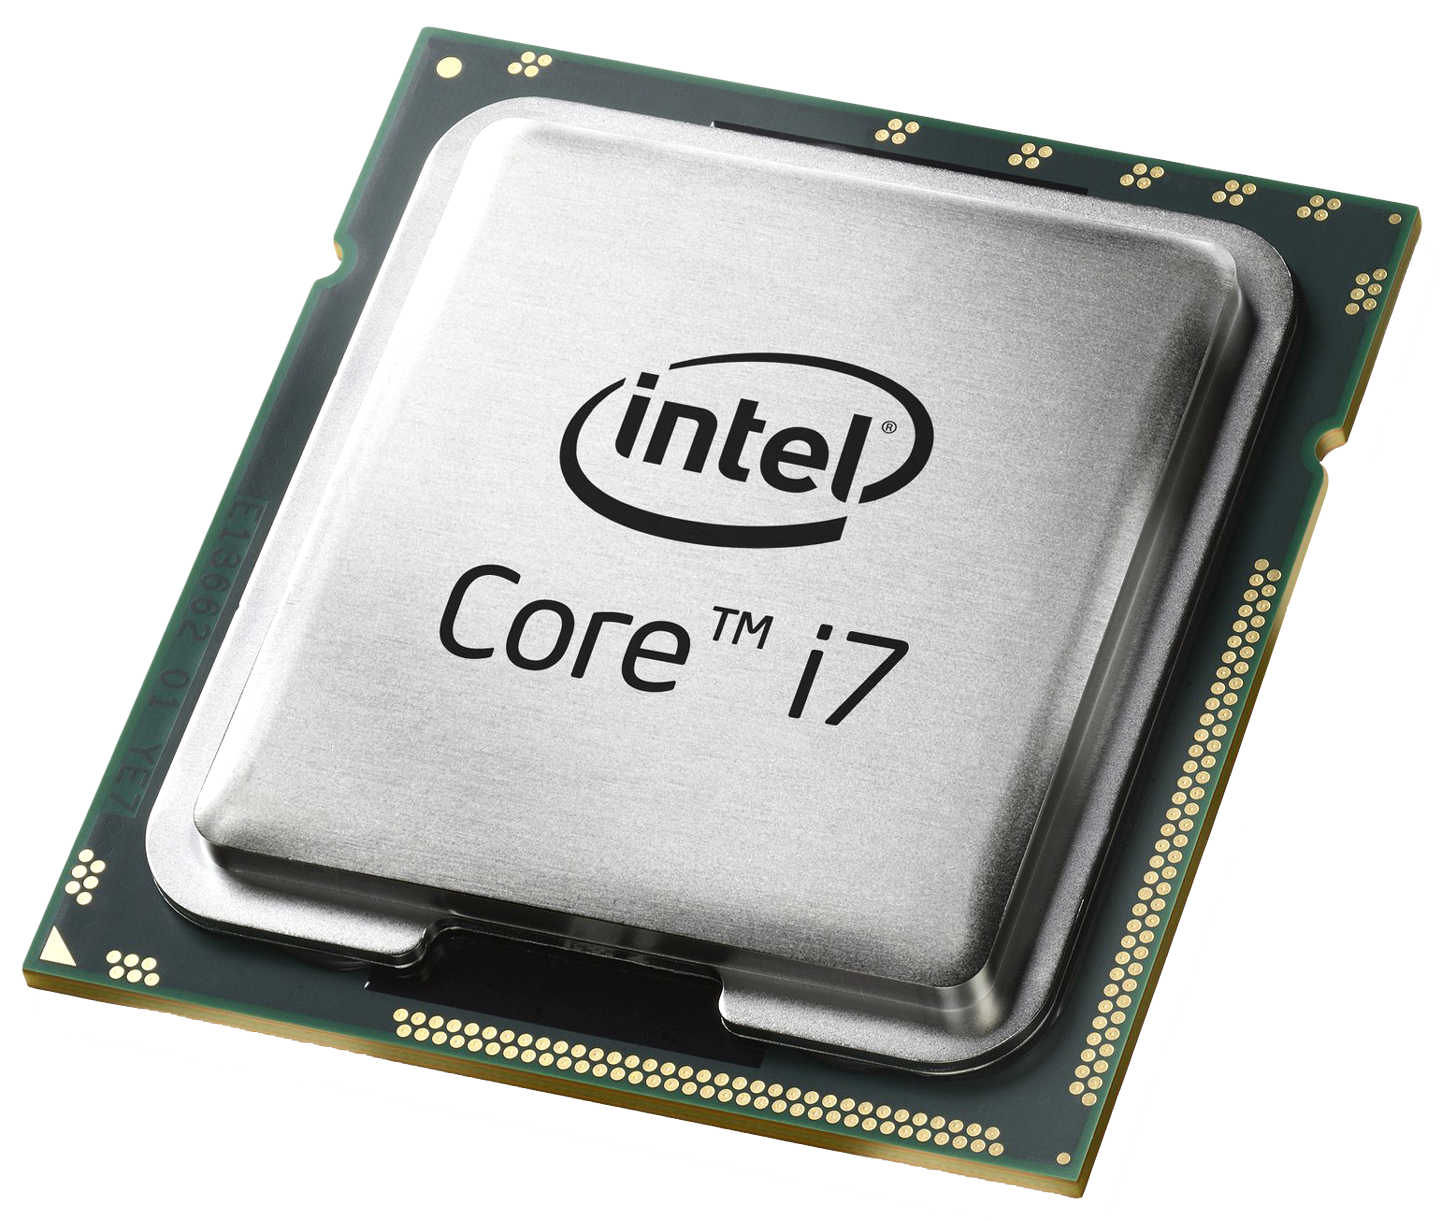
\includegraphics[width=0.3\textwidth]{../common/chapter_02/resources/01_cpu_intel.png}
    \captionof{figure}{Intel CPU}
\end{minipage}
Nun fragt man sich zurecht, wie die CPU denn solche Aufgaben bewältigen kann? Dazu muss man wissen, dass die CPU
selbst wiederum aus mehreren Teilen besteht, die alle eine bestimmte Aufgabe erfüllen. Es sind dies im Wesentlichen:
\begin{description}
    \item[Control unit] Diese Einheit steuert den ganzen Ablauf der CPU. Sie sagt den anderen Komponenten im Gerät und
    in der CPU selbst, was sie wann tun sollen und steuert so das ganze Gerät.\cite{wikipedia:cu}
    \item[Arithmetic logic unit] Wenn arithmetische oder logische Operationen durchgeführt werden sollen, dann ist diese
    Einheit wichtig. Wenn z.B. 4 + 5 gerechnet werden soll, dann wird die ALU damit beauftragt.\cite{wikipedia:alu}
    \item[Address generation unit] Will die CPU auf den Hauptspeicher zugreifen, dann wird in dieser Einheit die korrekte
    Adresse berechnet. Was das genau bedeutet wird im nächsten Abschnitt erklärt.\cite{wikipedia:agu}
\end{description}
Die CPU beinhaltet noch mehr solcher Einheiten, auf diese wird aber nun nicht mehr weiter eingegangen.
\subsection{Übung 1 - Zahlenspiel}
Es wird Zeit für die erste kleine Übung. Wir wollen darin das Verständnis stärken, wie Zahlen überhaupt in einem Computer
dargestellt werden und wie wir in der Lage sind, diese zu addieren.\\
Du hast sicher schon gehört, dass ein Computer mit 1en und 0en arbeitet.
TODO: Go on

\section{Exercise 1 - Let the drone fly} \lipsum[1]
\section{Exercise 1 - Let the drone fly} \lipsum[1]